\section{Testing and Results}




Out of interest, the here used dataset using only images labeled as "no\_mask"
and "ffp2", was used in another model found online. The code was written by
Adrian Rosebrock and uses the already pre-trained MobilNetV2 classifier
\cite{Rosebrock2020}. This would be the goto implementation in case one is focused
on making the classifier work and not creating one from scratch. The advantage
is, that this classifier has already been trained on a lot of different images,
which allows it to much easier adjust weights for new purposes as long as it
involves image classification. Repurposing this for a simple mask / no mask
detection is very simple and very accurate. Listing 2 and Figure
\ref{fig:mobilenetv2} show the performance of this model. It is very clear, that
the performance is exceptional considering the training and validation data. It
would remain to be seen, how the model performs on new images with very
different faces, but it is clear to say, that this model outperforms the one
created in this project by far.

\lstinputlisting[language=md,breaklines,caption={classification report},captionpos=b]{../code/classification_mobilenetv2.md}

\begin{figure}
    \centering
    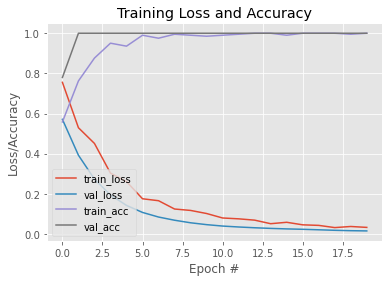
\includegraphics[width=0.4 \textwidth]{mobilenetv2_loss_and_acc.png}
    \caption{MobilNetV2 classifier - training results}
    \label{fig:mobilenetv2}
\end{figure}
